%tapered_extension
Moreover, there are other optional designs of tapered waveguides, which can be involved to improve the Fiber-to-Chip coupling ability. In following other possibilities of tapered structures are only delivered for reference and most of them will not be verified here.   \\
\subsubsection*{Hybrid tapered waveguides}%\\ 
\begin{figure}[!ht]
\centering
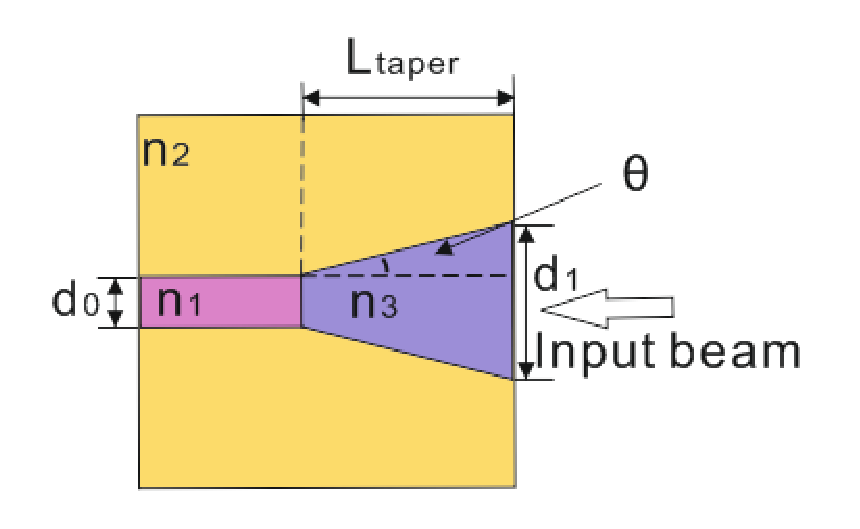
\includegraphics[width=0.7\textwidth]{bilder/tapered_waveguide_others}
\caption{Schema of a tapered waveguide combined with two different materials.}
\label{fig:tapered_waveguide_others}
\end{figure} 
In the other simulations of coupling between TLF and tapered waveguide there is another interesting result. If the taper is made from a proper material different from both guide and substrate, a more efficient coupling can be achieved comparing with previous designs.\\

\begin{figure}[!ht]
\centering
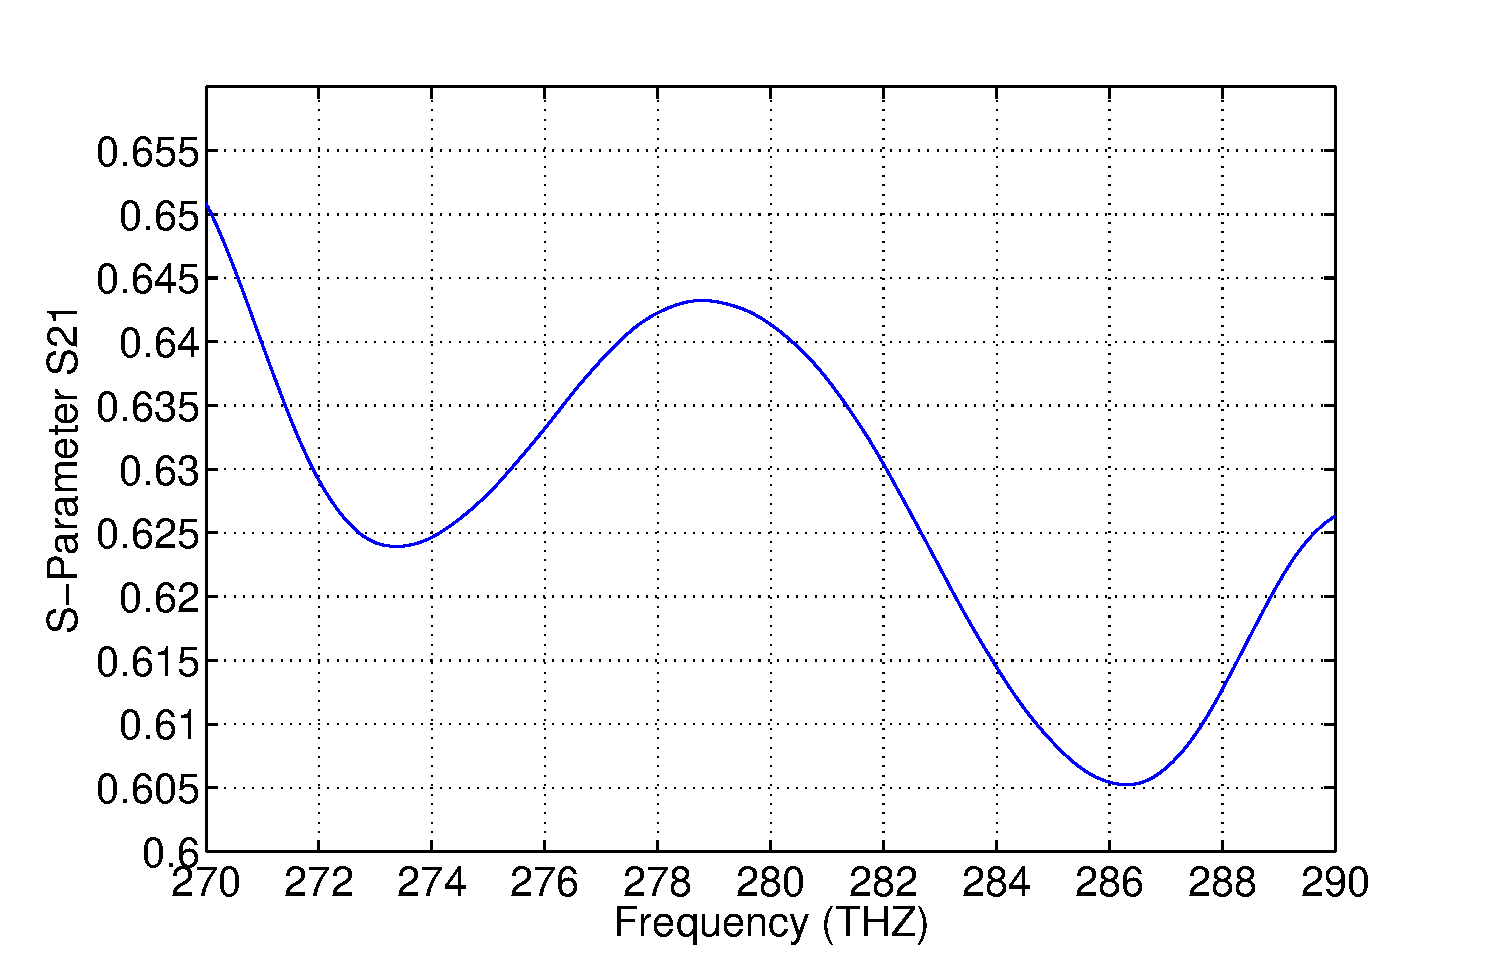
\includegraphics[width=0.7\textwidth]{bilder/s21_tapered_waveguide_others}
\caption{Coupling efficiency between TLF and the tapered waveguide combined with two different materials.}
\label{fig:tapered_waveguide_others_coupling}
\end{figure} 
For example, the taper is designed for $n=2.0$, $d_{1}=2\mu$m, $L_{taper}=5.5\mu$m and other configurations are same with those of the original simulation models. In this case the coupling efficiency reaches $63\%$ according to the simulation result in Fig. \ref{fig:tapered_waveguide_others_coupling}.  Because this design is not easy for fabrication, no more attention will be paid on it in this section.\\
   
\subsubsection*{Other tapered waveguides}
%\subsubsection*{Tapered plasmonic waveguides}%\\
Verhagen introduced in \cite{tapered_plasmonic_waveguides} a tapered plasmonic waveguide like Fig. \ref{fig:tapered_waveguide_plasmonic}, which included a thin tapered metal film. For transmission input beams can excite the surface plasmon polariton (SPP) wave, which is explained by quantum emission, provided by the metal/dielectric interfaces of the plasmonic waveguides. In \cite{tapered_plasmonic_waveguides} there is no result about coupling efficiency, but Verhagen's experiments exhibited that this structure can highly concentrate the incident power and has no cutoff behaviors along the taper.\\


Alonso-Ramos has provided in \cite{fiber_to_chip_grating_waveguides} an inversely tapered waveguide with gratings like Fig. \ref{fig:tapered_waveguide_grating}. The gratings of this waveguide are delicately designed to match the work mode: bloch mode. In \cite{fiber_to_chip_grating_waveguides} the author presented his achievement of $65.6\%$ coupling efficiency. \\

\begin{figure}[!ht]
\centering
\subfigure[Schema of a taperd plasmonic waveguide.]{
 	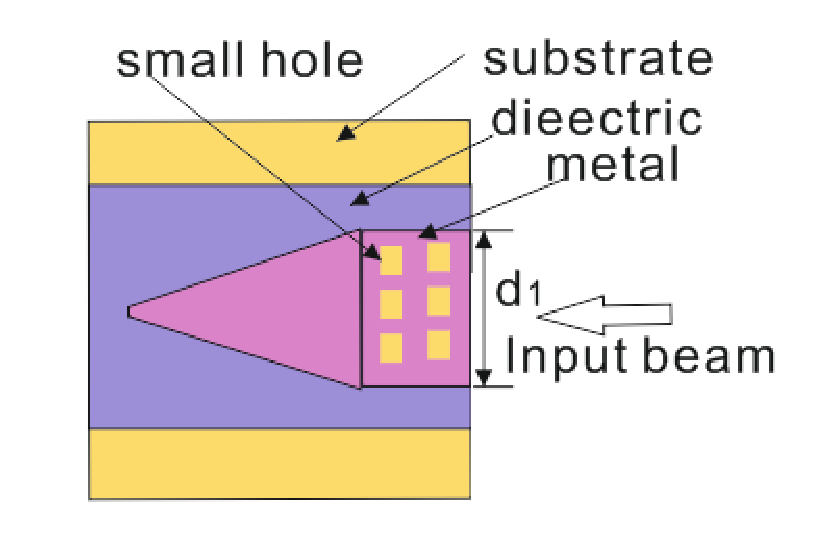
\includegraphics[width=0.48 \textwidth]{bilder/tapered_waveguide_plasmonic}
 	\label{fig:tapered_waveguide_plasmonic}
 	}
\subfigure[Schema of a taperd waveguide with grating.]{
 	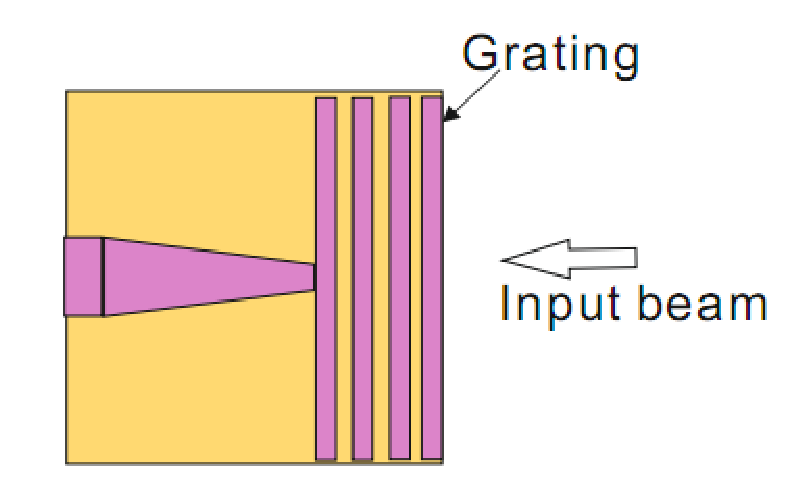
\includegraphics[width=0.48 \textwidth]{bilder/tapered_waveguide_grating}
 	\label{fig:tapered_waveguide_grating}
 	}
 \caption{Other tapered waveguide technigues.}

%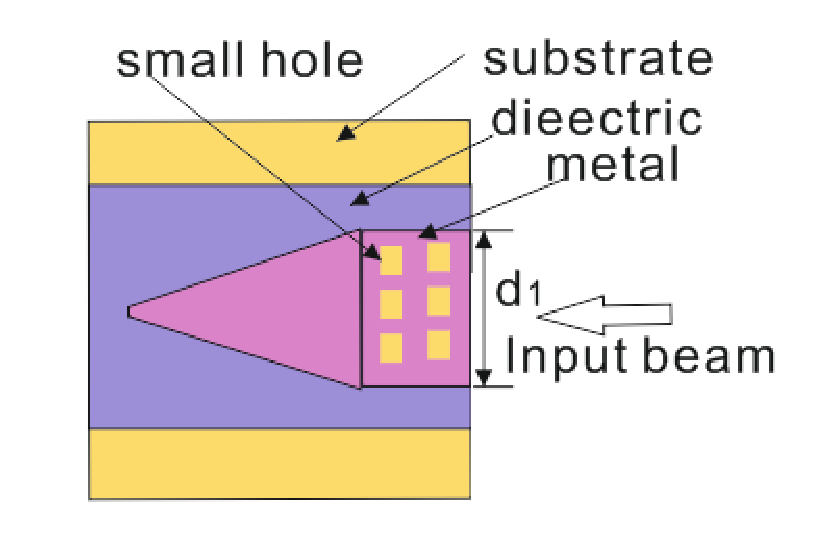
\includegraphics[width=0.65\textwidth]{bilder/tapered_waveguide_plasmonic}
%\caption{Schema of a taperd plasmonic waveguide.}
%\label{fig:tapered_waveguide_plasmonic}
%\end{figure}
%\subsubsection*{Grating tapered waveguides}%\\
%\begin{figure}[!ht]
%\centering
%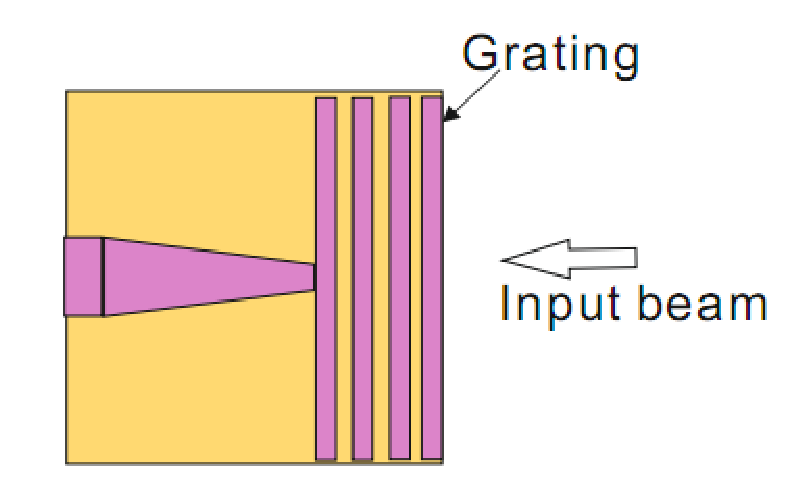
\includegraphics[width=0.65\textwidth]{bilder/tapered_waveguide_grating}
%\caption{Schema of a taperd waveguide with grating.}
%\label{fig:tapered_waveguide_grating}
\end{figure}
